\documentclass[10pt]{beamer}
\usetheme{jambro}

\title[]{Pensamento Econômico Contemporâneo - A escola monetarista ortodoxa}
\author[]{Paulo Victor da Fonseca}
\date{}

\hypersetup{
    colorlinks = true,
    urlcolor = teal,
    linkcolor = teal    
}
\usepackage[portuguese]{babel}
\usepackage{subfig}
\usepackage{emoji}

\begin{document}

\begin{frame}[plain]
    \titlepage{
        \begin{center}
            \begin{minipage}{0.8\textwidth}
                \centering
            \end{minipage}
        \end{center}}
\end{frame}

\begin{frame}{Sumário}
    \tableofcontents
\end{frame}

\section{Teoria do ciclo de negócios de equilíbrio}
\begin{frame}{Teoria do ciclo de negócios de equilíbrio}
    \begin{itemize}
        \item Abordagem Keynesiana de ciclo de negócios: caracterizada por várias rigidezes e fricções que impedem flexibilidade de salários e preços.
        \bigskip
        \item Consequentemente, no curto prazo, mercados não se equilibram e PIB pode desviar significativamente do nível potencial por períodos consideráveis.
        \bigskip
        \item Monetaristas: crítica aos Keynesianos por subestimarem a importância de distúrbios monetários como a principal fonte de instabilidade agregada.
        \bigskip
        \item 1970s nova abordagem de flutuações agregadas iniciada por Lucas: \textcolor{purple}{abordagem de equilíbrio aos ciclos de negócios}.
        \bigskip
        \item Esta nova abordagem foi uma ruptura significativa com análise de ciclos de negócios Keynesiana onde flutuações do PIB eram vistas como fenômenos de desequilíbrio.
    \end{itemize}
\end{frame}

\begin{frame}{Teoria do ciclo de negócios de equilíbrio}
    \begin{itemize}
        \item Fundamentos da teoria de ciclos de negócios de Lucas:
        \bigskip
        \begin{itemize}
            \item Preços e quantidades de equilíbrio exibem uma relação sistemática entre taxa de variação de preços nominais (inflação) e nível real de produto.
            \bigskip
            \item Essa variante da curva de Phillips é derivada em um arcabouço no qual todas as formas de `ilusão monetária' são rigorosamente excluídas: todos os preços representam equilíbrios de mercados, todos os agentes são otimizadores dados objetivos e expectativas, e expectativas são formadas de maneira ótima.
            \bigskip
            \item Movimentos nos preços resultam de um \textcolor{purple}{deslocamento de demanda relativa} ou de um \textcolor{purple}{deslocamento nominal (monetário)}.
            \bigskip
            \item Este comportamento resulta em não-neutralidade da moeda, ou uma curva de Phillips.
            \bigskip
            \item Ao mesmo tempo, mantem-se resultados clássicos: neutralidade da moeda no longo prazo, ou independência de magnitudes reais e nominais.
        \end{itemize}
    \end{itemize}
\end{frame}

\begin{frame}{Teoria do ciclo de negócios de equilíbrio}
    \begin{itemize}
        \item Lucas demonstrou que neste arcabouço Walrasiano, variações monetárias têm consequências reais mas, apenas, `porque agentes não conseguem discriminar perfeitamente entre deslocamentos reais e monetários'.
        \bigskip
        \item Portanto, não há um trade-off entre inflação e produto real que seja explorável.
        \bigskip
        \item `A curva de Phillips emerge não como um fato empírico inexplicável mas, sim, como uma característica central da solução de um sistema de equilíbrio geral' (Lucas, 1972).
    \end{itemize}
\end{frame}

\begin{frame}{Teoria do ciclo de negócios de equilíbrio}
    \begin{itemize}
        \item \textcolor{purple}{Ciclos de negócios são movimentos correlacionados serialmente ao redor de um componente de tendência do produto real que não são explicados por movimentos na disponibilidade de fatores de produção} (Lucas, 1975).
        \bigskip
        \item Associados às flutuações no PIB estão co-movimentos entre diferentes séries temporais agregadas: preços, consumo, lucros, investimento, agregados monetários, produtividade e taxas de juros.
        \bigskip
        \item Estas regularidades são tais que Lucas (1977) afirma que os ciclos econômicos são todos similares (exceção à Grande Depressão).
        \bigskip
        \item Para Lucas, \textcolor{purple}{o caráter recorrente dos ciclos de negócios é fundamental}.
    \end{itemize}
\end{frame}

\begin{frame}{Teoria do ciclo de negócios de equilíbrio}
    \begin{quote}
        Na medida em que ciclos de negócios possam ser vistos como instâncias repetidas de eventos essencialmente similares, é razoável tratar agentes como reagindo a mudanças cíclicas como `risco', ou assumir que suas expectativas são \emph{racionais}, que possuem arranjos razoavelmente estáveis para coletar e processar informações, e que eles utilizam essas informações para prever o futuro em uma maneira estável, livre de vieses sistemáticos e facilmente corrigíveis.
    \end{quote}
    \begin{flushright}
    (Lucas, 1977).
    \end{flushright}
\end{frame}

\begin{frame}{Teoria do ciclo de negócios de equilíbrio}
    \begin{itemize}
        \item Lucas fornece uma explicação `novo-clássica' monetarista para os ciclos de negócios como um fenômeno de equilíbrio ($\times$ noção de desequilíbrio).
        \bigskip
        \item Para Lucas, o problema central da macroeconomia é estabelecer uma abordagem onde distúrbios monetários podem causar flutuações de produto real ao mesmo tempo em que isto não implique a existência de oportunidades lucrativas persistentes, recorrentes e inexploradas - como ocorre em modelos Keynesianos caracterizados por rigidezes de preços e expectativas não-racionais.
    \end{itemize}
\end{frame}

\begin{frame}{Teoria do ciclo de negócios de equilíbrio}
    \begin{itemize}
        \item Teoria monetária de equilíbrio de ciclos de negócios (MEBCT) de Lucas:
        \bigskip
        \begin{enumerate}
            \item Hipótese de expectativas racionais - Muth (1961).
            \bigskip
            \item Hipótese da taxa natural - Friedman (1968).
            \bigskip
            \item Metodologia de equilíbrio geral Walrasiano.
        \end{enumerate}
        \bigskip
        \item Com equilíbrio contínuo de mercado devido às hipóteses de flexibilidade de preços e salários, as flutuações na MEBCT são descritas como equilíbrios competitivos.
        \bigskip
        \item Como choques monetários podem criar flutuações neste arcabouço?
        \bigskip
        \item Modelo clássico: agentes com informação perfeita e, portanto, variações na oferta de moeda são estritamente neutras.
        \bigskip
        \item O comportamento pró-cíclico e de liderança da moeda observado empiricamente sugere que a moeda não é neutra (ignorando a possibilidade de causalidade reversa).
    \end{itemize}
\end{frame}

\begin{frame}{Teoria do ciclo de negócios de equilíbrio}
    \begin{itemize}
        \item Modelo de Lucas: permite não-neutralidade da moeda ao estender modelo clássico de agentes racionais e otimizadores onde todos os mercados continuamente se equilibram com \textcolor{purple}{informação imperfeita} - conhecido como \textcolor{blue}{teoria das percepções errôneas} (\emph{misperceptions theory}).
        \bigskip
        \item Cabe ressaltar que a ideia de instabilidade ser o resultado de percepções errôneas induzidas por distúrbios monetários é, também, uma característica da análise de Friedman (1968) da curva de Phillips.
    \end{itemize}
\end{frame}

\begin{frame}{Teoria do ciclo de negócios de equilíbrio}
    \begin{itemize}
        \item O modelo de Lucas (1975) de Teoria Monetária de Equilíbrio dos Ciclos de Negócios é caracterizado por:
        \bigskip
        \begin{enumerate}
            \item Preços e quantidades determinados em um equilíbrio competitivo.
            \bigskip
            \item Agentes com expectativas racionais.
            \bigskip
            \item Informação imperfeita - não só o futuro é incerto mas, também, nenhum agente é perfeitamente informado acerca do estado corrente da economia.
        \end{enumerate}
        \bigskip
        \item \textcolor{purple}{A hipótese de que a oferta agregada depende de preços relativos é central à teoria novo-clássica de flutuações de produto e emprego}.
    \end{itemize}
\end{frame}

\begin{frame}{Teoria do ciclo de negócios de equilíbrio}
    \begin{itemize}
        \item Choques de demanda agregada não-antecipados (resultantes, principalmente, de variações não-antecipadas na oferta de moeda) que afetam a economia causam erros nas expectativas de preços (formadas racionalmente) e resultam em um desvio do produto e emprego com relação aos níveis de equilíbrio (natural) de longo prazo (informação completa).
        \bigskip
        \item Estes erros são feitos por firmas e trabalhadores em um ambiente de informação incompleta - interpretam de forma errônea variações no nível geral de preços como se fossem mudanças de preços relativos.
    \end{itemize}
\end{frame}

\begin{frame}{Teoria do ciclo de negócios de equilíbrio}
    \begin{itemize}
        \item Modelo micro neoclássico: (i) curva de oferta positivamente inclinada - preço relativo aumenta, produção aumenta; (ii) inflação pura não afeta quantidade produzida; (iii) informação perfeita.
        \bigskip
        \item Evidência empírica: produto agregado aumenta quando nível geral de preços aumenta (curta de oferta agregada de curto prazo é positivamente inclinada no espaço $P-Y$).
        \bigskip
        \item Isso significa que a resposta agregada de milhares de produtores a um aumento do nível generalizado de preços é positiva, mesmo que indivíduos maximizadores de lucros não deveriam se comportar dessa forma.
        \bigskip
        \item \textcolor{purple}{Agentes racionais deveriam responder apenas a variáveis reais e seu comportamento deveria ser invariante a variáveis nominais}.
    \end{itemize}
\end{frame}

\begin{frame}{Teoria do ciclo de negócios de equilíbrio}
    \begin{itemize}
        \item A explicação novo-clássica é atribuída à informação imperfeita acerca de preços relativos dos agentes (trabalhadores, famílias e firmas).
        \bigskip
        \item Se os agentes se acostumaram a um mundo de preços estáveis, tenderão a interpretar um aumento no preço de oferta do bem (ou serviço) que produzem como um aumento de preços relativos e, portanto, irão aumentar produção.
        \bigskip
        \item Portanto, um aumento inesperado ou não-antecipado do nível de preços irá surpreender os agentes que interpretarão, de forma errônea, a informação como um aumento de preços relativos.
        \bigskip
        \item Se todos os agentes cometem o mesmo erro, observaremos um aumento agregado no produto, correlacionado a um aumento do nível geral de preços.
        \bigskip
        \item Como o modelo de Lucas é `monetarista', o aumento generalizado de preços é causado por um aumento na oferta de moeda e, então, observamos uma correlação positiva entre moeda e produto - não-neutralidade da moeda.
    \end{itemize}
\end{frame}

\begin{frame}{Teoria do ciclo de negócios de equilíbrio}
    \begin{itemize}
        \item Considere uma economia em uma posição inicial na qual produto e emprego estejam em seus níveis naturais.
        \bigskip
        \item Suponha um distúrbio monetário não-antecipado - aumento generalizado de preços e em todos os mercados (\textcolor{purple}{ilhas}).
        \bigskip
        \item Firmas possuem informação acerca de preços apenas em um número limitado de mercados nos quais transacionam.
        \bigskip
        \item Se firmas individuais interpretam o aumento de preços de seus bens como um aumento de preços relativos de seus produtos, irão aumentar sua produção.
        \bigskip
        \item Trabalhadores também possuem informação incompleta - interpretam um aumento de salário nominal (relativo ao valor esperado) como um aumento de salário real e, portanto, aumentam a oferta de trabalho (Lucas e Rapping, 1969).
    \end{itemize}
\end{frame}

\begin{frame}{Teoria do ciclo de negócios de equilíbrio}
    \begin{itemize}
        \item No modelo de Friedman os trabalhadores são `enganados'.
        \bigskip
        \item O modelo de Lucas não requer nenhum tipo de assimetria de informação entre trabalhadores e firmas.
        \bigskip
        \item Firmas e trabalhadores são propensos a cometer erros de expectativas e, portanto, respondem positivamente a percepções errôneas de aumentos generalizados de preços com aumentos na oferta de bens e trabalho.
        \bigskip
        \item Produto agregado e emprego, portanto, aumentam temporariamente - acima dos níveis naturais.
        \bigskip
        \item Quando os agentes percebem que não houve variações de preços relativos, emprego e produto agregado retornam aos níveis naturais de equilíbrio de longo prazo.
    \end{itemize}
\end{frame}

\begin{frame}{Teoria do ciclo de negócios de equilíbrio}
    \begin{itemize}
        \item \textcolor{purple}{Modelo de Lucas: choques monetários são a principal causa de instabilidade agregada e a ideia é baseada na confusão por parte dos agentes entre movimentos de preços relativos e generalizados}.
        \bigskip
        \item A oferta de produto em qualquer instante do tempo pode ser decomposta em um componente permanente (secular) e um componente cíclico:
        \begin{equation}
            Y_t = Y_t^n + Y_t^c.
            \label{eq1}
        \end{equation}
        \bigskip
        \item O componente permanente do PIB reflete o crescimento subjacente da economia e segue a linha de tendência dada por:
        \begin{equation}
            Y_t^n = \lambda + \phi_t.
            \label{eq2}
        \end{equation}
    \end{itemize}
\end{frame}

\begin{frame}{Teoria do ciclo de negócios de equilíbrio}
    \begin{itemize}
        \item O componente cíclico é dependente da surpresa de preços e do desvio do produto com relação à taxa natural do período anterior:
        \begin{equation}
            Y_t^c = \alpha[P_t - \mathbb{E}(P_t|\Omega_{t-1})] + \beta(Y_{t-1}-Y_{t-1}^n).
            \label{eq3}
        \end{equation}
        \bigskip
        \item O termo defasado do produto em (\ref{eq3}) reflete o fato de que desvios do produto com relação à tendência serão mais que transitórios dada a influência de uma variedade de mecanismos de propagação.
        \bigskip
        \item O coeficiente $\beta > 0$ determina a velocidade com a qual o produto retorna ao seu nível natural após o choque.
    \end{itemize}
\end{frame}

\begin{frame}{Teoria do ciclo de negócios de equilíbrio}
    \begin{itemize}
        \item A combinação da HER e função de oferta agregada implica que produto e emprego irão flutuar aleatoriamente ao redor dos seus níveis naturais.
        \bigskip
        \item Portanto, hipóteses adicionais são necessárias para explicar porque durante o ciclo de negócio o produto e emprego permanecem persistentemente acima ou abaixo dos valores de tendência por uma sucessão de períodos temporais.
        \bigskip
        \item Os movimentos serialmente correlacionados observados entre produto e emprego (i.e., níveis de produto e emprego em qualquer período são correlacionados com valores precedentes) são explicados na literatura de várias formas.
    \end{itemize}
\end{frame}

\begin{frame}{Teoria do ciclo de negócios de equilíbrio}
    \begin{itemize}
        \item Estas explicações (mecanismos de propagação) incluem: produto defasado, efeitos aceleradores de investimento, defasagens informacionais e durabilidade de bens de capital, existência de contratos inibindo ajustes imediatos e custos de ajustamentos.
        \bigskip
        \item Por exemplo: firmas se deparam com custos tanto para contratar quanto para demitir empregados - custos associados à entrevistas e treinamentos de novos empregados, etc.
        \bigskip
        \item Consequentemente, as respostas ótimas podem ser ajustar os níveis de produto e emprego ao longo do tempo de maneira gradual seguindo um choque não-antecipado.
    \end{itemize}
\end{frame}

\begin{frame}{Teoria do ciclo de negócios de equilíbrio}
    \begin{itemize}
        \item Pelas equações (\ref{eq1}), (\ref{eq2}) e (\ref{eq3}) temos a \textcolor{purple}{relação de oferta agregada de Lucas}:
        \begin{equation}
            Y_t = \lambda + \phi_t + \alpha[P_t - \mathbb{E}(P_t|\Omega_{t-1})] + \beta(Y_{t-1} - Y_{t-1}^n) + \varepsilon_t.
            \label{eq4}
        \end{equation}
    \end{itemize}
\end{frame}

\begin{frame}{Teoria do ciclo de negócios de equilíbrio}
    \begin{itemize}
        \item No modelo de Lucas, as ações dos agentes são não-ótimas \textcolor{purple}{ex post}, no entanto, no equilíbrio de expectativas racionais eles estão fazendo o melhor que podem dadas as informações (incompletas) que adquiriram.
        \bigskip
        \item Distúrbios monetários tem uma maior propensão a causar um efeito maior sobre as variavéis reais em países que apresentam estabilidade de preços.
        \bigskip
        \item Em países em que agentes estão habituados a inflação, choques monetários, provavelmente, não terão um impacto significativo sobre variáveis reais.
    \end{itemize}
\end{frame}

\begin{frame}{Teoria do ciclo de negócios de equilíbrio}
    \begin{itemize}
        \item Seja $\theta$ a fração de variância total nos preços individuais causada por variações nos preços relativos.
        \bigskip
        \item Portanto, quanto maior o valor de $\theta$, maior será a variabilidade observada nos preços atribuída pelos agentes a um choque real (i.e., preços relativos) e menor o peso para movimentos de inflação pura.
        \bigskip
        \item Podemos, então, modificar a curva de oferta agregada de Lucas:
        \begin{equation}
            Y_t = \lambda + \phi_t + \theta\alpha[P_t - \mathbb{E}(P_t|\Omega_{t-1})] + \beta(Y_{t-1} - Y_{t-1}^n) + \varepsilon_t.
            \label{eq5}
        \end{equation}
        \bigskip
        \item \textcolor{purple}{Pela equação (\ref{eq5}), um choque monetário não-antecipado em países nos quais os agentes estão habituados a estabilidade de preços levará a um impacto significativo no produto real}.
    \end{itemize}
\end{frame}

\begin{frame}{Teoria do ciclo de negócios de equilíbrio}
    \begin{itemize}
        \item Modelo de ciclos de negócios de Lucas - resumo:
        \bigskip
        \begin{enumerate}
            \item Ciclos de negócios são gerados por choques monetários de demanda exógenos que transmitem sinais imperfeitos de preços para os agentes.
            \bigskip
            \item Agentes, em um mundo de informação imperfeita, respondem aos aumentos de preços com um aumento de oferta.
            \bigskip
            \item Quanto maior a variabilidade do nível geral de preços (menor a variação de preços atribuída por mudanças de preços relativos), menor será a resposta cíclica de produto a um distúrbio monetário.
        \end{enumerate}
        \bigskip
        \item Implicação de política: Uma política monetária apropriada eliminaria a principal fonte de instabilidade agregada.
        \bigskip
        \item Portanto, novos-clássicos advogam em favor de políticas sob regras na condução de políticas de estabilização.
    \end{itemize}
\end{frame}

\section{Implicações de política econômica}
\subsection{Proposição de ineficácia da política econômica}

\begin{frame}{Proposição de ineficácia da política econômica}
    \begin{itemize}
        \item \textcolor{purple}{Ineficácia de política econômica}: medidas de política monetária completamente antecipadas pelos agentes serão inefetivas em influenciar o nível de produto e emprego mesmo no curto prazo - \textcolor{blue}{super-neutralidade da moeda} (Sargent e Wallace 1975, 1976).
        \bigskip
        \item Considere uma economia operando, incialmente, na intersecção tripla entre as curvas de demanda agregada ($AD_0$), oferta agregada de curto prazo ($SRAS_0$) e oferta agregada de longo prazo ($LRAS$).
        \bigskip
        \item Neste ponto, o nível de preços ($P_0$) é inteiramente antecipado (níveis de preços observado e esperado coincidem) e produto e emprego estão nos níveis naturais de equilíbrio de longo prazo.
    \end{itemize}
\end{frame}

\begin{frame}{Proposição de ineficácia da política econômica}
    \begin{figure}
        \centering
        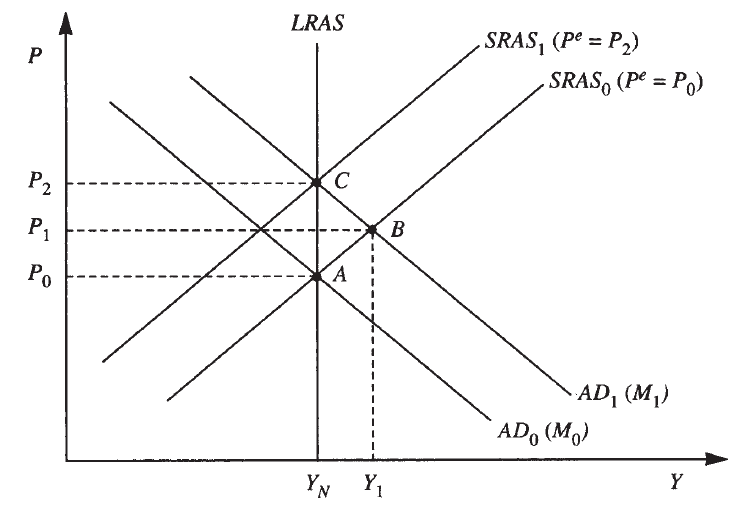
\includegraphics[width=0.6\textwidth]{./figures/aula12_fig1.PNG}
        \caption{Efeitos de políticas monetárias antecipadas e não-antecipadas. Fonte: Snowdon e Vane (2005).}
        \label{fig1}
    \end{figure}
\end{frame}

\begin{frame}{Proposição de ineficácia da política econômica}
    \begin{itemize}
        \item Suponha uma expansão monetária anunciada pelo BC.
        \bigskip
        \item Agentes racionais, então, incorporarão esta informação em seu processo de formação de expectativas e anteciparão completamente o efeito da expansão monetária sobre o nível generalizado de preços.
        \bigskip
        \item Produto e emprego permanecerão inalterados em seus níveis naturais.
        \bigskip
        \item O deslocamento da DA será inteiramente compensado por um deslocamento para cima da curva de AS de curto prazo - salários nominais aumentariam seguindo uma revisão de alta das expectativas de preços.
        \bigskip
        \item Equilíbrio se move ao longo da curva de AS de longo prazo vertical - sem alterações de emprego e produto mesmo no curto prazo: moeda é super-neutra.
    \end{itemize}
\end{frame}

\begin{frame}{Proposição de ineficácia da política econômica}
    \begin{itemize}
        \item Considere, agora, uma expansão monetária não anunciada pelo BC.
        \bigskip
        \item Firmas e trabalhadores com informação imperfeita irão interpretar de forma errônea o aumento generalizado de preços como um aumento de preços relativos - aumento da oferta de produto e emprego.
        \bigskip
        \item Curva de DA desloca para a direita e o equilíbrio de CP é dado pela intersecção com a curva $SRAS_0$.
        \bigskip
        \item Como vimos:
        \begin{equation}
            Y_t = Y_t^n + \alpha[P_t - P_t^e].
            \label{eq6}
        \end{equation}
        \bigskip
        \item Portanto, o produto desviará do nível natural como consequência do desvio do nível de preços com relação ao nível esperado - erros expectacionais.
    \end{itemize}
\end{frame}

\begin{frame}{Proposição de ineficácia da política econômica}
    \begin{itemize}
        \item Qualquer aumento/queda no produto/emprego será apenas temporário.
        \bigskip
        \item Quando agentes perceberem que não houve mudanças de preços relativos, produto e emprego retornam para níveis naturais.
        \bigskip
        \item À medida que os indivíduos ajustam completamente suas expectativas de preços, a curva de AS de curto prazo desloca para a esquerda.
        \bigskip
        \item Cabe ressaltar que, independente se a expansão monetária é antecipada ou não-antecipada:
        \bigskip
        \begin{enumerate}
            \item No primeiro caso que vimos, o processo novo-clássico de ajustamento corresponde ao caso monetarista de longo prazo.
            \bigskip
            \item No segundo caso, o processo corresponde ao caso monetarista de curto prazo.
        \end{enumerate}
    \end{itemize}
\end{frame}

\begin{frame}{Proposição de ineficácia da política econômica}
    \begin{itemize}
        \item Se a oferta monetária é determinada pelas autoridades de acordo com alguma regra `conhecida', então, os formuladores de política serão incapazes de influenciar produto e emprego mesmo no CP ao adotarem uma política monetária sistemática, já que pode ser antecipada pelos agentes.
        \bigskip
        \begin{enumerate}
            \item Regra exógena de taxa de crescimento da oferta monetária.
            \bigskip
            \item Oferta monetária determinada por regras de feedback (e.g., respostas a variações no desemprego e produto).
        \end{enumerate}
    \end{itemize}
\end{frame}

\begin{frame}{Proposição de ineficácia da política econômica}
    \begin{itemize}
        \item A proposição de ineficácia de política pode ser expressa formalmente utilizando a equação modificada linear de Friedman-Phelps:
        \begin{equation}
            \pi_t = \pi_t^e - \phi (U_t - U_t^n) + \phi \varepsilon_t^s,
            \label{eq7}
        \end{equation}
        onde $\varepsilon_t^s$ representa um choque de oferta exógeno (média zero) - \textcolor{purple}{cost-push inflation}.
        \bigskip
        \item Portanto:
        \begin{equation}
            U_t = U_t^n - \frac{1}{\phi}(\pi_t - \pi_t^e) + \varepsilon_t^s.
            \label{eq8}
        \end{equation}
        \bigskip
        \item A relação estrutural entre inflação e taxa de crescimento da moeda é dada por:
        \begin{equation}
            \pi_t = \dot{M}_t + \varepsilon_t^d,
            \label{eq9}
        \end{equation}
        onde $\varepsilon_t^d$ representa choques de demanda não-antecipados (média zero) - \textcolor{purple}{demand-pull inflation}.
    \end{itemize}
\end{frame}

\begin{frame}{Proposição de ineficácia da política econômica}
    \begin{itemize}
        \item Seja $\dot{M}_t^e$ a taxa esperada de crescimento da oferta de moeda, a inflação de expectativas racionais será:
        \begin{equation}
            \pi_t^e = \dot{M}_t^e.
            \label{eq10}
        \end{equation}
        \bigskip
        \item Suponha uma autoridade monetária de tradição Keynesiana que tenta controlar o crescimento monetário.
        \bigskip
        \item De forma que cresça a uma taxa constante ($\lambda_0$) somada a uma proporção ($\lambda_1$) do desvio do desemprego com relação ao nível natural observado no período anterior.
        \bigskip
        \item Neste caso, a taxa de crescimento da moeda será:
        \begin{equation}
            \dot{M}_t = \lambda_0 + \lambda_1 (U_{t-1} - U_{t-1}^n) + \varepsilon_t^m,
            \label{eq11}
        \end{equation}
        $\varepsilon_t^m$ é um elemento aleatório ou não-antecipado de crescimento monetário.
    \end{itemize}
\end{frame}

\begin{frame}{Proposição de ineficácia da política econômica}
    \begin{itemize}
        \item A equação (\ref{eq11}) indica que a autoridade monetária opera sob uma regra monetária sistemática de feedback que pode ser prevista por parte de agentes econômicos racionais à medida que é incorporada em seu conjunto de informação ($\Omega$).
        \bigskip
        \item Portanto, agentes racionais terão expectativas de inflação baseadas na taxa esperada de crescimento monetário:
        \begin{equation}
        \dot{M}_t^e = \lambda_0 + \lambda_1(U_{t-1}-U_{t-1}^n).
        \label{eq12}
        \end{equation}
        \bigskip
        \item Subtraindo (\ref{eq12}) de (\ref{eq11}):
        \begin{equation}
            \dot{M}_t - \dot{M}_t^e = \varepsilon_t^m.
            \label{eq14}
        \end{equation}
    \end{itemize}
\end{frame}

\begin{frame}{Proposição de ineficácia da política econômica}
    \begin{itemize}
        \item Portanto:
        \[
        \pi_t - \pi_t^e = \varepsilon_t^d + \varepsilon_t^m.
        \]
        \bigskip
        \item Temos então a seguinte representação em forma reduzida:
        \begin{equation}
            U_t = U_t^n - \frac{1}{\phi}(\varepsilon_t^m + \varepsilon_t^d) + \varepsilon_t^s.
            \label{eq14}
        \end{equation}
        \bigskip
        \item Note que o componente sistemático de crescimento monetário - que o BC tenta usar para impedir que o desemprego desvie do nível natural - não entra na equação.
        \bigskip
        \item \textcolor{purple}{O único componente da equação (\ref{eq14}) que a autoridade monetária pode influenciar diretamente é $\varepsilon_t^m$, o componente aleatório de crescimento da moeda}.
    \end{itemize}
\end{frame}

\begin{frame}{Proposição de ineficácia da política econômica}
    \begin{itemize}
        \item Modelo de Sargent e Wallace - equação (\ref{eq14}): desemprego desvia da taxa natural como resultado de choques não previsíveis de demanda e de oferta e choques não-antecipados no crescimento da moeda. Regras sistemáticas de política monetária são ineficazes.
        \bigskip
        \item Evidência empírica da proposição de ineficácia da política monetária:
        \bigskip
        \begin{enumerate}
            \item Barro (1977, 1978) - usando um método de estimação em dois estágios para dados da economia EUA no período 1941-1976, Barro encontra evidência em favor da proposição.
            \bigskip
            \item Mishkin (1982) e Gordon (1982) encontraram evidências que sugerem que tanto choques não-antecipados quanto antecipados de política monetária afetam produto e emprego.
        \end{enumerate}
        \bigskip
        \item Mesmo que a evidência empírica seja inconclusiva, não parece favorável à visão de que política monetária sistemática não tenha efeitos reais.
    \end{itemize}
\end{frame}

\begin{frame}{Proposição de ineficácia da política econômica}
    \begin{itemize}
        \item Críticas:
        \bigskip
        \begin{enumerate}
            \item Buiter (1980): modelos teóricos podem ser construídos nos quais mudanças completamente antecipadas na taxa de crescimento da moeda tenha efeitos reais.
            \bigskip
            \item Política fiscal é não neutra, mesmo no mais clássico dos sistemas.
            \bigskip
            \item Em modelos que permitem desequilíbrios de mercado, choques antecipados de política monetária terão efeitos reais via mecanismos IS-LM/AD-AS.
            \bigskip
            \item Fischer (1977), Phelps e Taylor (1977) e Taylor (1980): modelos que incorporam contratos salariais multi-períodos e expectativas racionais e a política monetária é não-neutra (novo-Keynesianos).
            \bigskip
            \item Hahn (1982): por que estimular DA quando a economia está no equilíbrio de pleno emprego?
        \end{enumerate}
    \end{itemize}
\end{frame}

\subsection{Custos reais de desinflação}
\begin{frame}{Custos reais de desinflação}
    \begin{itemize}
        \item Escola novo-clássica compartilha a visão monetarista de que a inflação é, essencialmente, um fenômeno monetário propagado por crescimento monetário excessivo.
        \bigskip
        \item Desacordo substancial quanto aos custos reais da desinflação existem entre economistas.
        \bigskip
        \item A perda em termos de produto que uma economia é sujeita para reduzir a inflação é conhecida como \textcolor{purple}{taxa de sacrifício}.
    \end{itemize}
\end{frame}

\begin{frame}{Custos reais de desinflação}
    \begin{itemize}
        \item \textcolor{purple}{Modelos Keynesianos}: taxa de sacrifício tende a ser elevada, mesmo com expectativas racionais, dado o ajuste viscoso de preços e salários a reduções de DA.
        \bigskip
        \begin{enumerate}
            \item Dado ajuste gradual de preços, um impulso deflacionário leva, inevitavelmente, a perdas reais significativas que podem ser prolongadas por \textcolor{blue}{efeito histerese} - recessão causa a taxa natural de desemprego a aumentar (Cross, 1988; Gordon, 1988).
            \bigskip
            \item Alguns Keynesianos, portanto, defendem o uso de políticas de renda como medidas auxiliares para acompanhar a contração monetária como forma de aumentar a eficiência das políticas de desinflação.
        \end{enumerate}
    \end{itemize}
\end{frame}

\begin{frame}{Custos reais de desinflação}
    \begin{itemize}
        \item \textcolor{purple}{Modelos monetaristas}: desemprego aumenta após uma contração monetária, a magnitude e duração dependem de alguns fatores:
        \bigskip
        \begin{enumerate}
            \item Grau da contração monetária.
            \bigskip
            \item Adaptações institucionais.
            \bigskip
            \item Velocidade com que agentes ajustam suas expectativas com relação às taxas futuras de inflação.
        \end{enumerate}
        \bigskip
        \item O fator crítico é a responsividade das expectativas com relação à mudança de regime monetário.
        \bigskip
        \item Isto, por sua vez, implica que a credibilidade e reputação da autoridade monetária tem um papel fundamental em determinar a razão de sacrifício.
    \end{itemize}
\end{frame}

\begin{frame}{Custos reais de desinflação}
    \begin{itemize}
        \item \textcolor{purple}{Modelos novo-clássicos:} mudanças anunciadas/antecipadas de política monetária não tem efeito sobre produto e emprego, mesmo no curto prazo, caso a política seja crível.
        \bigskip
        \item \textcolor{blue}{Portanto, a autoridade monetária pode, em princípio, reduzir a taxa de inflação sem os custos associados em termos de produto e emprego previstos por modelos Keynesianos e monetaristas}.
        \bigskip
        \item Isto é, a razão de sacrifício é zero!
        \bigskip
        \item ``\emph{Em um mundo de Sargent-Wallace, o Fed pode eliminar inflação simplesmente anunciando que irá expandir a oferta de moeda a uma taxa compatível com a estabilidade de preços}'' (Gordon, 1978).
        \bigskip
        \item Dada a ausência de custos de emprego-produto, novos-clássicos argumentam que autoridades podem anunciar uma redução drástica na taxa de expansão monetária para reduzir a inflação à meta estabelecida (não é necessário ajuste gradual como em modelos monetaristas).
    \end{itemize}
\end{frame}

\begin{frame}{Custos reais de desinflação}
    \begin{itemize}
        \item Para que uma desinflação ocorra com uma razão de sacrifício igual a zero, o público deve acreditar que a autoridade monetária está comprometida a conduzir a contração monetária anunciada!
        \bigskip
        \item Se os anúncios de política não apresentam credibilidade, então, as expectativas inflacionárias não irão cair o suficiente para impedir que a economia apresente custos em termos de produto e emprego.
        \bigskip
        \item A questão de credibilidade de políticas está associada com o problema de \textcolor{purple}{inconsistência temporal (ou dinâmica)}.
    \end{itemize}
\end{frame}

\subsection{Inconsistência temporal, credibilidade e regras monetárias}
\begin{frame}{Inconsistência temporal, credibilidade e regras monetárias}
    \begin{itemize}
        \item Argumentos monetaristas contra políticas ativistas discricionárias propostas por Keynesianos e em favor de uma regra monetária:
        \bigskip
        \begin{enumerate}
            \item Restrições informacionais dos formuladores de política.
            \bigskip
            \item Problemas associados a hiatos temporais e previsões.
            \bigskip
            \item Incerteza a respeito do tamanho dos multiplicadores fiscais e monetários.
            \bigskip
            \item Consequências inflacionárias de reduzir desemprego abaixo do nível natural.
            \bigskip
            \item Descrença no processo político comparado às forças de mercado.
        \end{enumerate}
        \bigskip
        \item A contribuição novo-clássica é a proposição de ineficácia de política de Lucas-Sargent-Wallace.
    \end{itemize}
\end{frame}

\begin{frame}{Inconsistência temporal, credibilidade e regras monetárias}
    \begin{itemize}
        \item Em 1977, Kydland e Prescott forneceram uma reformulação do caso contra políticas discricionárias.
        \bigskip
        \item Modelo novo-clássico onde o formulador de política econômica encontra-se em um jogo dinâmico estratégico com agentes racionais e forward-looking do setor privado.
        \bigskip
        \item Neste arcabouço, uma política monetária discricionária leva a um resultado de equilíbrio que envolve um \textcolor{purple}{viés inflacionário}.
    \end{itemize}
\end{frame}

\begin{frame}{Inconsistência temporal, credibilidade e regras monetárias}
    \begin{itemize}
        \item Kydland e Prescott: crítica à abordagem convencional, inspirada em Tinbergen (1952).
        \bigskip
        \item A abordagem convencional consiste em três pontos básicos:
        \bigskip
        \begin{enumerate}
            \item Formulador de política econômica deve especificar seus objetivos de política econômica (e.g., baixa inflação e desemprego).
            \bigskip
            \item Dada a função de bem-estar que deseja maximizar, um conjunto de instrumentos (fiscais ou monetários) é escolhido para atingir estas metas.
            \bigskip
            \item Formulador, então, utiliza de um modelo econômico de forma a determinar os valores dos instrumentos em seus valores ótimos.
        \end{enumerate}
        \bigskip
        \item Esta abordagem normativa diz como formuladores de política econômica devem agir, em um contexto de teoria do controle ótimo, para identificar a política ótima de maneira a alcançar o melhor resultado, dadas as preferências da autoridade.
    \end{itemize}
\end{frame}

\begin{frame}{Inconsistência temporal, credibilidade e regras monetárias}
    \begin{itemize}
        \item Kydland e Prescott argumentam que não é possível que a teoria do controle ótimo (TCO) seja aplicável a planejamento econômico quando as expectativas são racionais.
        \bigskip
        \item A TCO é útil no contexto das ciências físicas mas no caso de sistemas sociais a questão é mais complicada.
        \bigskip
        \item Os agentes de um sistema social são inteligentes que tentarão antecipar as ações de política.
        \bigskip
        \item Como resultado, sistemas econômicos dinâmicos onde os formuladores de política estão em um contexto de sequências de ações ao longo de um período de tempo, políticas discricionárias não resultam em uma função objetivo social sendo otimizada.
        \bigskip
        \item Este paradoxo aparente é resultado do fato de que `o planejamento econômico não é um jogo contra natureza mas, sim, contra agentes econômicos racionais'.
    \end{itemize}
\end{frame}

\begin{frame}{Inconsistência temporal, credibilidade e regras monetárias}
    \begin{itemize}
        \item O argumento de Kydland e Prescott tem implicações importantes para a condução da política monetária e para a estrutura institucional mais provável para gerar credibilidade com relação ao objetivo de manter uma baixa taxa de inflação.
        \bigskip
        \item Quando os agentes são forward-looking, um problema de política emerge como um jogo dinâmico entre o setor privado e e autoridade monetária.
    \end{itemize}
\end{frame}

\begin{frame}{Inconsistência temporal, credibilidade e regras monetárias}
    \begin{itemize}
        \item Suponha que o governo formule o que considera ser uma política ótima e, então, anuncia aos agentes privados.
        \bigskip
        \item Se esta política é crível, então, nos períodos subsequentes, manter a política anunciada pode não continuar sendo ótimo dado que, na nova situação, o governo tem um incentivo para alterar a política ótima anunciada anteriormente.
        \bigskip
        \item A diferença entre a otimalidade ex ante e ex post da política é o que chamamos de \textcolor{purple}{inconsistência dinâmica (ou temporal)}.
        \bigskip
        \item Uma política ótima computada em $t$ é dinamicamente inconsistente se o período $t + n$ implica uma política ótima diferente - Blackburn (1992).
        \bigskip
        \item Kydland e Prescott demonstraram como políticas que apresentam inconsistência dinâmica irão enfraquecer, de forma significativa, a credibilidade de políticas anunciadas.
    \end{itemize}
\end{frame}

\begin{frame}{Inconsistência temporal, credibilidade e regras monetárias}
    \begin{itemize}
        \item Para demonstrar que os planos ótimos apresentam inconsistência temporal, consideraremos um jogo estratégico entre autoridades monetárias e agentes econômicos privados.
        \bigskip
        \item Para isso utilizaremos o modelo de Lucas de surpresas monetárias para representar o trade-off de curto prazo entre inflação e desemprego para demonstrar como um equilíbrio consistente irá apresentar um viés inflacionário.
        \bigskip
        \item No modelo de Kydland e Prescott, políticas discricionárias são incapazes de alcançar um equilíbrio ótimo.
        \bigskip
        \item Vamos assumir que o BC pode controlar a taxa de inflação perfeitamente, que todos os mercados estão continuamente em equilíbrio e os agentes possuem expectativas racionais.
    \end{itemize}
\end{frame}

\begin{frame}{Inconsistência temporal, credibilidade e regras monetárias}
    \begin{itemize}
        \item Neste modelo, o desemprego pode ser reduzido por uma surpresa inflacionária positiva:
        \begin{equation}
            U_t = U_t^n + \psi(\pi_t^e - \pi_t).
            \label{eq15}
        \end{equation}
        \bigskip
        \item A equação (\ref{eq15}) representa a restrição com que o formulador de política econômica se depara.
        \bigskip
        \item Como mencionado, as expectativas são racionais:
        \[
        \pi_t^e = \mathbb{E}(\pi_t|\Omega_{t-1}).
        \]
        \bigskip
        \item Assuma uma função objetivo social ($S$) que racionalize a escolha política:
        \begin{equation}
            S = S(\pi_t, U_t), \qquad S'(\pi_t)<0, \quad S'(U_t)<0.
            \label{eq16}
        \end{equation}
    \end{itemize}
\end{frame}

\begin{frame}{Inconsistência temporal, credibilidade e regras monetárias}
    \begin{itemize}
        \item A função objetivo social (\ref{eq16}) indica que inflação e desemprego são `maus econômicos', dado que uma redução leva a um aumento de bem estar social.
        \bigskip
        \item Uma política consistente ótima busca maximizar (\ref{eq16}) sujeito à restrição imposta pela curva de Phillips (\ref{eq15}).
        \bigskip
        \item A Figura \ref{fig2} ilustra o trade-off da curva de Phillips para duas taxas de inflação esperadas.
        \bigskip
        \item As linhas de contorno da função objetivo social são indicadas por $S_1, S_2, S_3, S_4$.
        \bigskip
        \item Dado que inflação e desemprego são `maus econômicos', $S_1>S_2>S_3>S_4$, e a forma das curvas de indiferença implicam que a taxa socialmente preferida de inflação é igual a zero.
    \end{itemize}
\end{frame}

\begin{frame}{Inconsistência temporal, credibilidade e regras monetárias}
    \begin{figure}
        \centering
        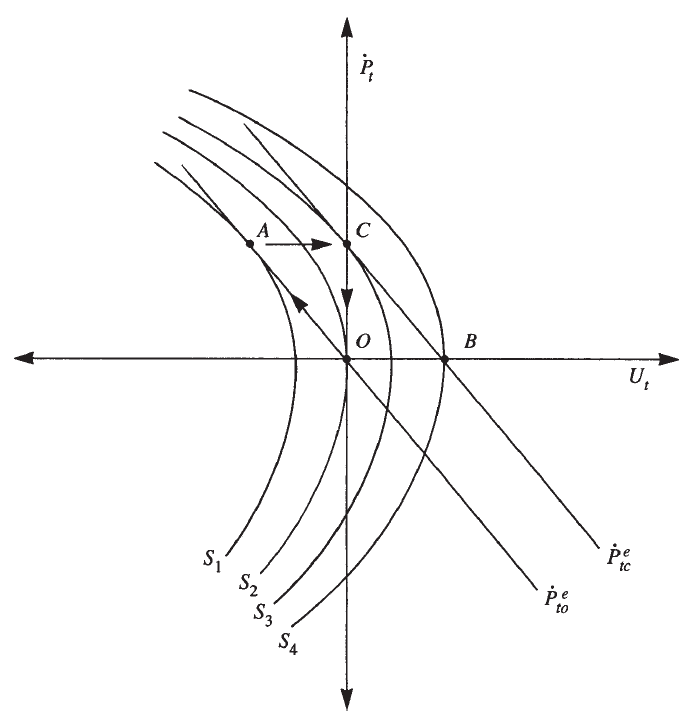
\includegraphics[width=0.4\textwidth]{./figures/aula12_fig2.PNG}
        \caption{Equilíbrio ótimo e consistente. Fonte: Snowdon e Vane (2005).}
        \label{fig2}
    \end{figure}
\end{frame}

\begin{frame}{Inconsistência temporal, credibilidade e regras monetárias}
    \begin{itemize}
        \item Na Figura \ref{fig2}, todos os pontos ao longo do eixo vertical são posições potenciais de equilíbrio, dado que em pontos como $O$ e $C$ o desemprego está no seu nível natural e os agentes estão corretamente prevendo a inflação.
        \bigskip
        \item As curvas de indiferença indicam que a posição ótima (equilíbrio consistente) é no ponto $O$ onde $\pi_t = 0$ e $U_t = U_t^n$.
        \bigskip
        \item Embora a autoridade monetária possa determinar a taxa de inflação, a posição das curvas de Phillips dependerão das expectativas inflacionárias dos agentes econômicos privados.
        \bigskip
        \item Nesta situação, um equilíbrio dinamicamente consistente é alcançado no ponto de tangência entre a curva de indiferença $S_3$ e a curva de Phillips que passa pelo ponto $C$.
        \bigskip
        \item Fica evidente que este equilíbrio dinamicamente consistente é sub-ótimo.
    \end{itemize}
\end{frame}

\begin{frame}{Inconsistência temporal, credibilidade e regras monetárias}
    \begin{itemize}
        \item Em um jogo dinâmico, cada jogador escolhe uma estratégia que indique como irão se comportar à medida que informações são recebidas durante o jogo.
        \bigskip
        \item A estratégia escolhida por um jogador particular depende da percepção que eles tem das prováveis estratégias adotadas pelos outros participantes e, também, como eles esperam que os outros jogadores sejam influenciados por suas próprias estratégias.
        \bigskip
        \item Em um jogo dinâmico, cada jogador maximiza sua função objetivo sujeito à perpecção que tem das estratégias adotadas por outros jogadores.
    \end{itemize}
\end{frame}

\begin{frame}{Inconsistência temporal, credibilidade e regras monetárias}
    \begin{itemize}
        \item Um jogo entre o governo (autoridades monetárias) e agentes privados é um exemplo de um \textcolor{purple}{jogo não-cooperativo de Stackelberg}.
        \bigskip
        \item Jogos de Stackelberg possuem um estrutura hierárquica, com o jogador dominante agindo como um líder e os outros participantes reagindo à estratégia adotada pelo líder.
        \bigskip
        \item No jogo de política monetária descrito por Kydland e Prescott, o governo (BC) é o jogador dominante.
        \bigskip
        \item Quando o governo decide sua política ótima, irá levar em consideração a provável reação dos `seguidores' (agentes privados).
    \end{itemize}
\end{frame}

\begin{frame}{Inconsistência temporal, credibilidade e regras monetárias}
    \begin{itemize}
        \item Em um jogo de Stackelberg, a menos que o líder se comprometa com a política anunciada, a política ótima será inconsistente temporalmente dado que o governo pode aumentar seu pay-off mudando sua estratégia ex-post.
        \bigskip
        \item Como o setor privado incorpora esta informação, \textcolor{purple}{o equilíbrio de consistência temporal será um equilíbrio de Nash}.
        \bigskip
        \item Nesta situação, cada jogador percebe corretamente que estão fazendo o melhor que podem, dadas as ações dos outros jogadores, com o líder abdicando de seu papel dominante.
    \end{itemize}
\end{frame}

\begin{frame}{Inconsistência temporal, credibilidade e regras monetárias}
    \begin{itemize}
        \item Suponha que a economia esteja, inicialmente, no equilíbrio subótimo de consistência temporal - ponto $C$ na Figura \ref{fig2}.
        \bigskip
        \item Para mover a economia para a posição ótima indicada pelo ponto $O$, as autoridades monetárias anunciam uma meta de inflação zero que será alcançada reduzindo a taxa de crescimento da moeda de $\dot{M}_c$ para $\dot{M}_0$.
        \bigskip
        \item Se este anúncio é crível e aceitado pelos agentes privados, eles irão revisar para baixo suas expectativas inflacionárias, deslocando a curva de Phillips para baixo.
        \bigskip
        \item Uma vez que os agentes adaptaram suas expectativas, qual garantia eles terão de que o BC não irá abdicar de sua promessa e causar uma surpresa inflacionária?
    \end{itemize}
\end{frame}

\begin{frame}{Inconsistência temporal, credibilidade e regras monetárias}
    \begin{itemize}
        \item Como é evidente pela Figura \ref{fig2}, a política ótima para as autoridades é dinamicamente inconsistente.
        \bigskip
        \item Se usarem de seus poderes de discrição, eles podem aumentar a taxa de expansão monetária para criar uma surpresa inflacionária e, assim, a economia pode atingir o ponto $A$ que é claramente superior ao ponto $O$.
        \bigskip
        \item No entanto, esta posição não é sustentável, dado que no ponto $A$ o desemprego está abaixo do nível natural e $\pi_t>\pi_t^e$.
        \bigskip
        \item Agentes racionais irão perceber que foram `enganados' e, então, a economia irá retornar ao equilíbrio de consistência dinâmica no ponto $C$.
        \bigskip
        \item Note que neste ponto não há incentivos para as autoridades tentarem estimular a economia de forma a reduzir o desemprego - uma vez no ponto $C$, tal tentativa irá reduzir o bem-estar.
        \bigskip
        \item Ou seja, fosse este o caso, a economia se moveria para uma curva de indiferença social inferior.
    \end{itemize}
\end{frame}

\begin{frame}{Inconsistência temporal, credibilidade e regras monetárias}
    \begin{itemize}
        \item Em resumo, apesar de termos $A > 0 > C$, apenas o ponto $C$ é dinamicamente consistente.
        \bigskip
        \item O ponto $A$ é insustentável dado que o desemprego está abaixo do nível natural.
        \bigskip
        \item No ponto $O$, as autoridades tem um incentivo para `trapacear' de forma a atingir um nível mais elevado de bem estar social (temporário).
        \bigskip
        \item Portanto, se as autoridades monetárias tem poder de discrição, elas terão um incentivo para desviar das políticas anunciadas.
        \bigskip
        \item Portanto, \textcolor{purple}{políticas anunciadas que sejam inconsistentes dinamicamente não serão críveis}.
        \bigskip
        \item Como os outros jogadores conhecem a função objetivo da autoridade monetária, eles não irão ajustar suas expectativas inflacionárias em resposta a políticas anunciadas que não sejam críveis e, então, na ausência de regras que sejam `binding', a economia não poderá atingir a posição ótima mas dinamicamente inconsistente no ponto $O$.
    \end{itemize}
\end{frame}

\begin{frame}{Inconsistência temporal, credibilidade e regras monetárias}
    \begin{itemize}
        \item O equilíbrio não-cooperativo de Nash, indicado pelo ponto $C$, demonstra que políticas discricionárias produzem um resultado subótimo que envolve um viés inflacionário.
        \bigskip
        \item Dado que agentes racionais podem antecipar a estratégia das autoridades monetárias que possuem poder de discrição, eles irão antecipar um nível de inflação mais elevado $\pi_{tc}^e$.
        \bigskip
        \item Portanto, formuladores de política deverão ofertar uma inflação que seja igual à expectativa do setor privado para impedir um estrangulamento do produto agregado.
        \bigskip
        \item \textcolor{purple}{Uma política ótima que não seja crível, dado a inconsistência temporal, não será, portanto, nem ótima nem factível}.
    \end{itemize}
\end{frame}

\begin{frame}{Inconsistência temporal, credibilidade e regras monetárias}
    \begin{itemize}
        \item Políticas discricionárias que selecionam a melhor política dada a situação existente irão levar a um resultado dinamicamente consistente mas, no entanto, subótimo.
        \bigskip
        \item A única forma de atingir a posição ótima, $O$, é quando as autoridades monetárias se comprometem a uma regra monetária não-contingente que seja consistente com a estabilidade de preços. 
    \end{itemize}
\end{frame}

\begin{frame}{Inconsistência temporal, credibilidade e regras monetárias}
    \begin{figure}
        \centering
        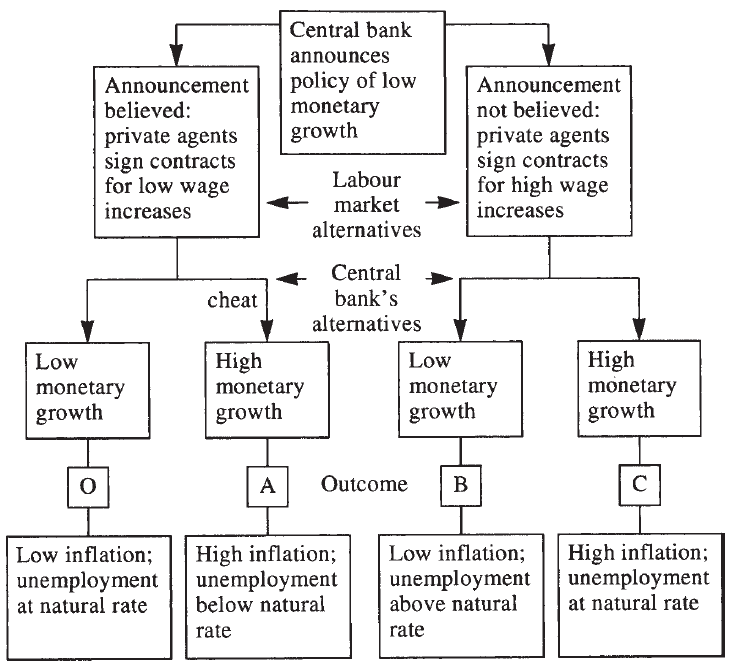
\includegraphics[width=0.5\textwidth]{./figures/aula12_fig3.PNG}
        \caption{Jogo entre autoridades monetárias e negociadores salariais. Fonte: Snowdon e Vane (2005).}
        \label{fig3}
    \end{figure}
\end{frame}

\begin{frame}{Inconsistência temporal, credibilidade e regras monetárias}
    \begin{itemize}
        \item Os quatro resultados possíveis que podem emergir no jogo não-cooperativo entre agentes privados e BC é representado na Figura \ref{fig3}, adaptada de Taylor (1985).
        \bigskip
        \item C - resultado de consistência temporal, O - resultado ótimo de baixa inflação com desemprego no nível natural.
        \bigskip
        \item O incentivo que o BC tem para estimular a economia devido à inconsistência temporal é indicado pelo resultado A.
        \bigskip
        \item A decisão de não validar uma elevada taxa de expectativa inflacionária e crescimento salarial elevado irá produzir uma recessão, como indicado em B.
    \end{itemize}
\end{frame}

\begin{frame}{Inconsistência temporal, credibilidade e regras monetárias}
    \begin{itemize}
        \item O problema de credibilidade identificado por Kydland e Prescott emerge mais claramente na situação de um jogo não-cooperativo de Stackelberg com informação completa de apenas uma rodada, onde o governo tem discrição com relação à política monetária.
        \bigskip
        \item No entanto, este é um jogo não-realista, dado que este jogo será repetido.
        \bigskip
        \item No caso de um jogo repetido (um super-jogo), o formulador de política é forçado a tomar uma visão de longo prazo, dado que as consequências futuras das decisões correntes de política irão influenciar a \textcolor{purple}{reputação} do formulador de política.
        \bigskip
        \item Nesta situação, o incentivo de desviar do plano anunciado é reduzido, porque ele se depara com um trade-off intertemporal entre os ganhos correntes de desviar e os custos futuros que emergirão inevitavelmente pela curva de Phillips.
    \end{itemize}
\end{frame}

\begin{frame}{Inconsistência temporal, credibilidade e regras monetárias}
    \begin{itemize}
        \item O problema de reputação é melhor analisado no modelo de inconsistência temporal de Barro e Gordon (1983).
        \bigskip
        \item Eles exploram as possibilidades de substituir a reputação do formulador de política por regras mais formais.
        \bigskip
        \item Se há consenso de que a inflação é, primariamente, determinada pelo crescimento da moeda, por que governos permitem uma expansão monetária excessiva?
        \bigskip
        \item No modelo de Barro-Gordon, um viés inflacionário resulta porque as autoridades monetárias não são restritas por regras.
        \bigskip
        \item No entanto, mesmo um governo explorando a discrição será influenciado por considerações de reputação no caso em que se depara com `punições' por parte dos agentes privados e, portanto, deve balancear os benefícios de desviar da política anunciada com os custos de inflação mais alta que caracteriza o equilíbrio discricionário.
    \end{itemize}
\end{frame}

\begin{frame}{Inconsistência temporal, credibilidade e regras monetárias}
    \begin{itemize}
        \item Neste caso, um tipo diferente de equilíbrio pode emergir, no qual o formulador de política renuncia dos ganhos de curto prazo de forma a manter uma reputação de longo prazo.
        \bigskip
        \item Dado este trade-off intertemporal entre os ganhos correntes (em termos de baixo desemprego e produto mais alto) e os custos futuros, \textcolor{purple}{o equilíbrio deste jogo dependerá da taxa de desconto do formulador de políticas}.
        \bigskip
        \item Quanto maior a taxa de desconto, mais próximo a solução de equilíbrio estará do equilíbrio de consistência temporal no modelo de Kydland-Prescott (ponto $C$).
        \bigskip
        \item Se a taxa de desconto é baixa, a posição de equilíbrio estará mais próxima do resultado ótimo de comprometimento de inflação zero.
        \bigskip
        \item Note que é a presença de um comprometimento prévio que distingue um regime monetário baseado em regras de um baseado em discrição.
    \end{itemize}
\end{frame}

\begin{frame}{Inconsistência temporal, credibilidade e regras monetárias}
    \begin{itemize}
        \item Um problema com a análise anterior é que os agentes privados não conhecem qual tipo de comportamento do governo se deparam, dado que eles possuem informação incompleta.
        \bigskip
        \item Dada a incerteza com respeito às intenções do governo, os agentes privados irão analisar cuidadosamente os vários sinais em forma de ações de política e anúncios.
        \bigskip
        \item Neste cenário, é difícil para os agentes privados distinguirem entre administrações de inflação zero das administrações de inflação alta.
        \bigskip
        \item Isso porque regimes de inflação alta tem um incentivo a se `passarem' por regimes de inflação zero.
    \end{itemize}
\end{frame}

\begin{frame}{Inconsistência temporal, credibilidade e regras monetárias}
    \begin{itemize}
        \item Mais recentemente, Svensson (1997) mostrou como as \textcolor{purple}{metas de inflação} emergiram como uma estratégia designada para eliminar o viés inflacionário inerente às políticas monetárias discricionárias.
        \bigskip
        \item A literatura de inconsistência temporal iniciada por Kydland-Prescott e Barro-Gordon assume que as autoridades monetárias, sob discrição, tentarão atingir uma meta de emprego implícita ao reduzir o desemprego abaixo da taxa natural, que eles acreditam ser ineficientemente elevada.
        \bigskip
        \item Este problema levou economistas a procurarem por arranjos monetários de credibilidade que ajudassem a resolver o problema de viés inflacionário.
    \end{itemize}
\end{frame}

\begin{frame}{Inconsistência temporal, credibilidade e regras monetárias}
    \begin{itemize}
        \item A \textcolor{blue}{`primeira melhor' solução} é corrigir as distorções do lado da oferta que estão fazendo com que a taxa natural de desemprego seja maior do que a desejada pelas autoridades monetárias, i.e., lidar com o problema em sua origem.
        \bigskip
        \item No entanto, se por alguma razão esta solução não é politicamente viável (e.g., sindicatos fortes), uma \textcolor{blue}{`segunda melhor' solução} envolve o comprometimento a uma regra de política monetária.
        \bigskip
        \item O segundo-melhor equilíbrio ainda pode ser atingido se atribuirmos às autoridades monetárias uma meta de emprego que seja igual à taxa natural.
        \bigskip
        \item Se nenhuma destas soluções é factível, então, a política será discricionária e a economia irá apresentar um viés inflacionário relativo ao segundo-melhor equilíbrio.
        \bigskip
        \item Svensson classifica o resultado discricionário (de inconsistência temporal) como a \textcolor{blue}{`quarta melhor' solução}.
    \end{itemize}
\end{frame}

\begin{frame}{Inconsistência temporal, credibilidade e regras monetárias}
    \begin{itemize}
        \item Melhorias do quarto-melhor resultado podem ser obtidas se modificarmos as preferências do banco central via delegação da política monetária a um \textcolor{purple}{banco central conservador com relação à inflação} (Rogoff, 1985).
        \bigskip
        \item Svensson argumenta que o regime de metas de inflação pode aproximar a economia da segunda-melhor solução.
    \end{itemize}
\end{frame}

\subsection{Independência do Banco Central}
\begin{frame}{Independência do Banco Central}
    \begin{itemize}
        \item O debate acerca de um Banco Central independente (BCI) tem sido bastante influenciada pelo pensamento novo-clássico.
        \bigskip
        \item Especialmente com relação às expectativas inflacionárias, inconsistência dinâmica, reputação e credibilidade.
        \bigskip
        \item Se o argumento de Kydland-Prescott de que polícias discricionárias levam a um viés inflacionário, é necessário estabelecer algum arranjo institucional que restrinja ações discricionárias - \textcolor{purple}{Banco Central Independente}.
    \end{itemize}
\end{frame}

\begin{frame}{Independência do Banco Central}
    \begin{itemize}
        \item Motivação teórica para BCI: hipótese da taxa natural implica que no longo prazo a taxa de inflação é independente do nível de desemprego e que políticas discricionárias, provavelmente, levam a um viés inflacionário.
        \bigskip
        \item Portanto, no LP com a inexistência de um trade-off explorável, autoridades monetárias que não sejam míopes deveriam selecionar uma posição na CPLP consistente com uma baixa taxa de inflação sustentável.
        \bigskip
        \item As teorias de inconsistência dinâmica oferecem uma explicação de porque inflação excessiva (moderada) será o resultado provável de um regime monetário no qual comprometimentos de longo prazo sejam ausentes.
    \end{itemize}
\end{frame}

\begin{frame}{Independência do Banco Central}
    \begin{itemize}
        \item \textcolor{purple}{A ênfase destes modelos na importância das instituições e regras para assegurar estabilidade de preços fornece uma forte defesa em favor do estabelecimento de bancos centrais independentes cujo poder de discrição é restrito por objetivos anti-inflacionários explicitos funcionando como dispositivos de comprometimento}.
        \bigskip
        \item Como o problema de credibilidade tem sua origem nos poderes de discrição das autoridades monetárias no que diz respeito à condução da política monetária, isto poderia ser contornado ao transferirmos a responsabilidade de políticas anti-inflacionárias para um banco central independente não-político.
        \bigskip
        \item Adicionalmente, um BCI irá se beneficiar de um `bônus de credibilidade', onde políticas desinflacionárias podem ser atingidas com uma baixa taxa de sacrifício.
    \end{itemize}
\end{frame}

\begin{frame}{Independência do Banco Central}
    \begin{itemize}
        \item Independência do Banco Central:
        \bigskip
        \begin{enumerate}
            \item \textcolor{purple}{Independência de objetivos}: o BC define seus próprios objetivos (i.e., independência política).
            \bigskip
            \item \textcolor{purple}{Independência de instrumentos}: o BC possui independência com respeito aos vários instrumentos de política monetária (i.e., independência econômica).
        \end{enumerate}
    \end{itemize}
\end{frame}

\begin{frame}{Independência do Banco Central}
    \begin{itemize}
        \item O  viés inflacionário associado ao problema de inconsistência dinâmica pode ser melhorado via `modificações nas preferências do Banco Central':
        \bigskip
        \begin{enumerate}
            \item \textcolor{purple}{Delegação da política monetária para um Banco Central conservador} - (Rogoff, 1985).
            \bigskip
            \item \textcolor{purple}{Adoção de contratos ótimos do Banco Central} - Walsh (1993, 1995).
        \end{enumerate}
    \end{itemize}
\end{frame}

\begin{frame}{Independência do Banco Central}
    \begin{itemize}
        \item Modelo de Rogoff: nomeação de um banqueiro central conservador com relação à inflação (atribui um peso relativo maior ao controle da inflação do que a sociedade de maneira geral).
        \bigskip
        \item O objetivo é assegurar que a inflação excessiva associada ao problema de inconsistência dinâmica seja mantida baixa em circunstâncias em que seria difícil estabelecer um comprometimento com inflação baixa.
        \bigskip
        \item De maneira geral, uma inflação média mais baixa e uma maior volatilidade do produto são implicados por este modelo.
        \bigskip
        \item No entanto, Alesina e Summers (1993) mostram que apenas a primeira predição aparece em dados cross-section.
    \end{itemize}
\end{frame}

\begin{frame}{Independência do Banco Central}
    \begin{itemize}
        \item O modelo de contratos ótimos de Walsh utiliza uma abordagem principal-agente e enfatiza a responsabilização do Banco Central.
        \bigskip
        \item Neste modelo, o BC tem independência de instrumentos, mas não de objetivos.
        \bigskip
        \item As recompensas ou penalizações ao BC são baseadas no seu desempenho com relação ao controle da inflação.
        \bigskip
        \item Exemplo aproximado: Reserve Bank of New Zealand.
        \bigskip
        \item Um ponto importante é a duração ótima do contrato de um banqueiro central:
        \bigskip
        \begin{enumerate}
            \item Nomeações de longa duração reduzem o papel de surpresas eleitorais - modelo partidário de Alesina.
            \bigskip
            \item Nomeações que sejam longas demais podem ser custosas se as preferências da sociedade estão sujeitas a mudanças frequentes.
        \end{enumerate}
        \bigskip
        \item A duração ótima deve balancear as vantagens em reduzir os efeitos eleitorais com a necessidade de assegurar que as preferências refletidas na política monetária sejam aquelas dos eleitores - Waller e Walsh (1996).
    \end{itemize}
\end{frame}

\begin{frame}{Independência do Banco Central}
    \begin{itemize}
        \item Evidência empírica (BCI): relação negativa entre BCI e inflação nas economias avançadas.
        \bigskip
        \item Dificuldade: construção de um índice de independência.
        \bigskip
        \item Alesina e Summers (1993): 
        \begin{enumerate}
            \item Habilidade do BC de selecionar seus objetivos de política sem interferência do governo.
            \bigskip
            \item Procedimento de seleção do presidente do BC.
            \bigskip
            \item Habilidade de utilização dos instrumentos monetários sem restrições.
            \bigskip
            \item Necessidade de que o BC financie déficits fiscais.
        \end{enumerate}
        
    \end{itemize}
\end{frame}

\begin{frame}{Independência do Banco Central}
    \begin{figure}
        \centering
        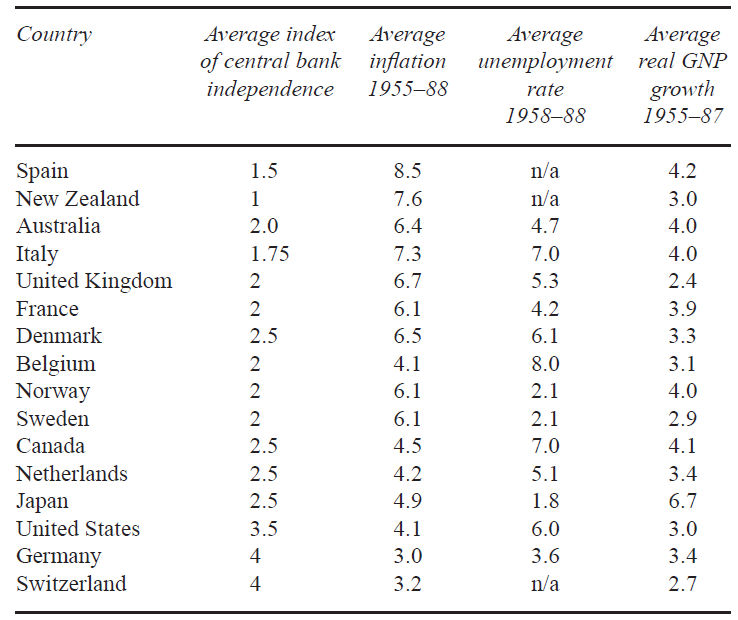
\includegraphics[width=0.5\textwidth]{./figures/aula12_fig4.PNG}
        \caption{Independência do Banco Central e performance econômica. Fonte: Alesina e Summers (1993).}
        \label{fig4}
    \end{figure}
\end{frame}

\begin{frame}{Independência do Banco Central}
    \begin{figure}
        \centering
        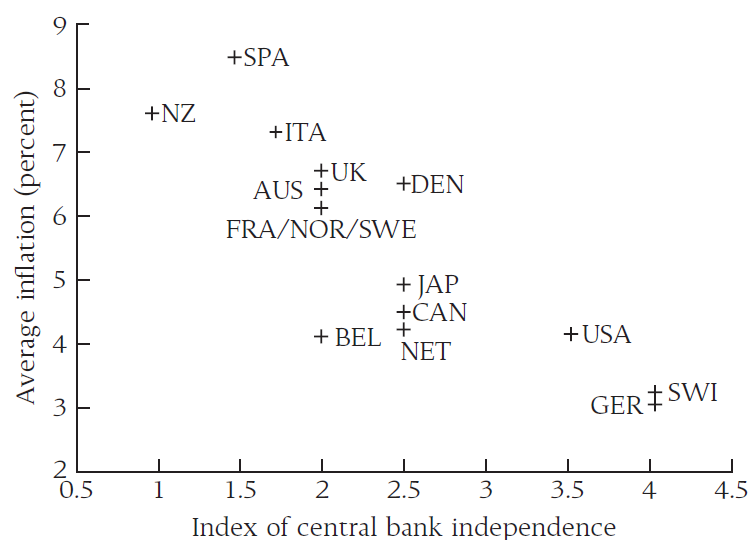
\includegraphics[width=0.6\textwidth]{./figures/aula12_fig5.PNG}
        \caption{Independência do Banco Central e inflação. Fonte: Alesina e Summers (1993).}
        \label{fig5}
    \end{figure}
\end{frame}

\begin{frame}{Independência do Banco Central}
    \begin{itemize}
        \item `Ao mesmo tempo em que a independência do Banco Central promove estabilidade de preços, não tem impactos mensuráveis sobre performance econômica real'.
        \bigskip
        \item Correlação negativa quase perfeita entre inflação e CBI.
        \bigskip
        \item \textcolor{purple}{Correlação não implica causalidade}.
        \bigskip
        \item A performance anti-inflacionária alemã pode ter uma maior relação com a aversão da sociedade com relação à inflação (pós-hiperinflação de 1923) do que com a existência de um BCI.
        \bigskip
        \item Neste caso, o BCI pode ser um efeito da aversão pública alemã à inflação ao invés de uma causa de inflação baixa.
        \bigskip
        \item Adesão de países a regimes monetários onde a política monetária é determinada por um BC anti-inflacionário - objetivo é restringir o poder dos formuladores de política econômica domésticos e ajudar a abaixar as expectativas inflacionárias.
    \end{itemize}
\end{frame}

\begin{frame}{Independência do Banco Central}
    \begin{itemize}
        \item Limitações dos resultados de Alesina e Summers (1993):
        \bigskip
        \begin{enumerate}
            \item Não é evidente que teorias de inconsistência dinâmica e delegação impliquem que uma maior independência irá produzir uma inflação mais baixa.
            \bigskip
            \item Correlação não implica causalidade: países em que a aversão dos cidadãos com relação à inflação é maior são mais propensos a isolar os BC das pressões políticas.
            \bigskip
            \item A relação empírica não é tão forte quanto aparenta ser: (i) não há nenhuma relação clara entre medidas legais de BCI e inflação média; (ii) as medidas usuais de independência parecem viesadas em favor de encontrar um link entre independência e inflação baixa (e.g., as medidas colocam pesos que indicam se o BC coloca inflação baixa como objetivo primário).
            \bigskip
            \item Mesmo que a independência seja a fonte da inflação baixa, o mecanismo que conecta os dois pode não envolver inconsistência dinâmica.
        \end{enumerate}
    \end{itemize}
\end{frame}

\begin{frame}{Independência do Banco Central}
    \begin{itemize}
        \item \textcolor{purple}{Nova macroeconomia política}: a literatura de `ciclos políticos de negócios' (CPN) sugere que CBI pode ajudar a reduzir o problema de distorções políticas na formulação de políticas macroeconômicas.
        \bigskip
        \item A imposição da HER não remove a importância de fatores políticos na análise de ciclos de negócios mas, em geral, a literatura CPN fornece mais argumentos em favor de tirar a condução da política monetária do poder de políticos eleitos - Alesina, Roubini e Cohen (1997); Drazen (2000).
    \end{itemize}
\end{frame}

\begin{frame}{Independência do Banco Central: objeções}
    \begin{enumerate}
        \item \textcolor{purple}{Trade-off flexibilidade $\times$ comprometimento}. CBI pode mitigar problemas de inconsistência dinâmica, no entanto, muitos acreditam que um BC com poder de discrição diante de grandes choques pode ser uma melhor alternativa às políticas baseadas em regras - visão de alguns Keynesianos (Stiglitz, Solow, Tobin).
        \bigskip
        \item \textcolor{purple}{Realismo do modelo}. Economistas que trabalharam em bancos centrais argumentam que a abordagem de teoria dos jogos não é útil e/ou realista para o comportamento dos BC. Além disso, Bernanke e Mishkin confirmam que `Bancos centrais nunca e em nenhum lugar aderem a regras estritas de crescimento monetário'.
    \end{enumerate}
\end{frame}

\begin{frame}{Independência do Banco Central}
    \begin{enumerate}
        \setcounter{enumi}{2}
        \item \textcolor{purple}{Falhas de coordenação: fiscal $\times$ monetária}. Potencial de CBI em gerar conflitos entre autoridades fiscal e monetária.
        \bigskip
        \begin{itemize}
            \item Em países em que isto levou a conflitos (EUA 1979-82), déficits fiscais elevados e taxas de juros reais elevadas emergiram.
            \bigskip
            \item O mix de política monetária rígida e política fiscal frouxa não é uma surpresa dadas as motivações predominantes de BCs e Tesouros Nacionais.
            \bigskip
            \item Bancos centrais tendem a enfatizar austeridade monetária e inflação baixa, autoridades fiscais sabem que aumentos nos gastos públicos e reduções de impostos são políticas atrativas.
            \bigskip
            \item Aos críticos, dizer que a inflação deve ser o objetivo primário do BC é bem diferente de tornar a inflação o único objetivo da política monetária.
            \bigskip
            \item \textcolor{blue}{`A credibilidade da política monetária não depende apenas da política monetária mas, também, do programa econômico por completo'} (Blackburn, 1992).
        \end{itemize}
    \end{enumerate}
\end{frame}

\subsection{Políticas microeconômicas para aumentar oferta agregada}
\begin{frame}{Políticas microeconômicas e oferta agregada}
    \begin{itemize}
        \item O papel da política monetária não é reduzir desemprego de forma permanente mas, sim, manter inflação baixa e estável.
        \bigskip
        \item Quais políticas adotar se o objetivo é aumentar produto/reduzir desemprego de maneira permanente?
        \bigskip
        \item Políticas microeconômicas que reduzem as distorções no mercado de trabalho - `primeira melhor solução' ao problema de viés inflacionário identificado por Kydland e Prescott (1977).
        \bigskip
        \item Desemprego é um resultado de equilíbrio que reflete decisões ótimas dos agentes econômicos - desemprego voluntário.
        \bigskip
        \item \textcolor{purple}{Medidas apropriadas de política são, então, aquelas que aumentam os incentivos microeconômicos para firmas e trabalhadores para ofertar mais trabalho e produto}.
    \end{itemize}
\end{frame}

\begin{frame}{Políticas microeconômicas e oferta agregada}
    \begin{itemize}
        \item Lucas (2003) - analisando performance dos EUA ao longo dos últimos 50 anos, concluiu que o potencial para ganhos de bem-estar que derivam de políticas de longo-prazo/de oferta excedem consideravelmente os ganhos potenciais de melhorias de políticas de estabilização de curto prazo.
        \bigskip
        \item Exemplo: para alguns economistas, o problema do desemprego na Europa não é, fundamentalmente, um problema de política monetária, mas um problema de lado de oferta - Euroesclerose.
        \bigskip
        \item Anos 1950 e 1960: estado de bem-estar social em economias europeias - desemprego médio mais baixo que EUA.
        \bigskip
        \item Anos 1980: reversão da evidência empírica.
    \end{itemize}
\end{frame}

\begin{frame}{Políticas microeconômicas e oferta agregada}
    \begin{itemize}
        \item Economistas atribuem essa performance ruim do mercado de trabalho europeu a mudanças institucionais que afetaram de maneira adversa a flexibilidade do mercado de trabalho.
        \bigskip
        \item Em particular, medidas relacionadas à quantidade e duração dos benefícios-desemprego, políticas de habitação que limitam mobilidade, legislação de salário mínimo e medidas de proteção ao emprego que aumenta os custos de contratação e desligamento, etc.
        \bigskip
        \item Solow (1998) e Modigliani (1996) aceitam a validade de alguns dos argumentos de lado de oferta, no entanto, veem que uma parte significativa do aumento no desemprego europeu tem origem nas políticas rígidas anti-inflacionárias que foram características das décadas recentes.
        \bigskip
        \item Portanto, a solução ao problema do desemprego europeu requer uma combinação de políticas de oferta micro-orientadas com políticas de estímulo de demanda agregada.
    \end{itemize}
\end{frame}

\subsection{Crítica de Lucas}
\begin{frame}{Crítica de Lucas}
    \begin{itemize}
        \item A teoria macro usa observações não experimentais sobre o comportamento passado da economia para entender seu funcionamento e fazer inferências futuras sobre o seu comportamento sob diferentes hipóteses a respeito da condução de políticas econômicas.
        \bigskip
        \item Bons modelos devem se ajustar bem aos dados passados e fornecer estimativas confiáveis a respeito do efeito de diferentes políticas sobre a economia.
        \bigskip
        \item Os modelos macroeconométricos Keynesianos dos anos 50 e 60 consistiam de `sistemas de equações' envolvendo variáveis endógenas e variáveis exógenas.
    \end{itemize}
\end{frame}

\begin{frame}{Crítica de Lucas}
    \begin{itemize}
        \item Tais modelos, seguindo Koopmans (1949), contem quatro tipos de equações - `equações estruturais':
        \bigskip
        \begin{enumerate}
            \item Identidades: equações que são verdadeiras por definição.
            \bigskip
            \item Equações que incorporam regras institucionais: e.g., agendas de impostos.
            \bigskip
            \item Equações que especificam restrições tecnológicas: e.g., funções de produção.
            \bigskip
            \item Equações comportamentais: descrevem a forma com que indivíduos/grupos respondem ao ambiente econômico (e.g., ajustes salariais, consumo, investimento e funções de demanda por moeda).
        \end{enumerate}
    \end{itemize}
\end{frame}

\begin{frame}{Crítica de Lucas}
    \begin{itemize}
        \item Modelo FMP (Federal Reserve - MIT - Penssylvania University) construído por Ando e Modigliani.
        \bigskip
        \item Modelo usado para predição e testar o impacto de choques estocásticos.
        \bigskip
        \item Dados históricos usados para estimar o modelo e, então, modelo utilizado para analisar as possíveis consequências de políticas alternativas.
        \bigskip
        \item O modelo Keynesiano típico era baseado na abordagem IS/LM-AS/AD combinado com uma curva de Phillips.
        \bigskip
        \item O comportamento deste modelo depende dos valores estimados para os coeficientes das variáveis.
    \end{itemize}
\end{frame}

\begin{frame}{Crítica de Lucas}
    \begin{itemize}
        \item \textcolor{purple}{Crítica de Lucas}: a prática estabelecida de utilizar modelos macroeconométricos de larga escala para avaliar as consequências de cenários alternativos de política não é confiável - estas simulações são baseadas na hipótese de que os parâmetros do modelo permaneçam inalterados quando há uma mudança de condução de política - Lucas (1976).
        \bigskip
        \item Cabe ressaltar que Keynes já havia argumentado com Tinbergen que os parâmetros dos modelos de equações simultâneas não eram invariantes.
    \end{itemize}
\end{frame}

\begin{frame}{Crítica de Lucas}
    \begin{itemize}
        \item Exemplo: função consumo Keynesiana $C = \alpha + \beta(Y-T)$.
        \bigskip
        \item Os parâmetros $(\alpha, \beta)$ irão depender das decisões ótimas que agentes econômicos tomaram no passado, dadas suas funções utilidade.
        \bigskip
        \item Ou seja, estes parâmetros foram determinados durante um processo de otimização anterior que são diretamente influenciados pelo regime de política particular prevalente naquele período.
        \bigskip
        \item Lucas: não podemos utilizar estes modelos para motivos de predição.
        \bigskip
        \item Os parâmetros de modelos macroeconométricos de larga escala podem não permanecer invariantes a mudanças de política - agentes ajustam suas expectativas e comportamento ao novo ambiente.
    \end{itemize}
\end{frame}

\begin{frame}{Crítica de Lucas}
    \begin{itemize}
        \item Modelos macroeconométricos devem, então, levar em consideração o fato de que qualquer mudança de política irá sistematicamente alterar a estrutura do modelo - agentes racionais se adaptam.
        \bigskip
        \item Como os modelos Keynesianos tradicionais não incorporavam isso, qualquer recomendação de política baseada nestas simulações seriam erradas.
        \bigskip
        \item A crítica de Lucas implica que a construção de modelos macroeconométricos devem ser reconsideradas por completo, de forma que as equações sejam estruturais ou comportamentais.
        \bigskip
        \item A crítica de Lucas contribuiu para a abordagem metodológica adotada nos anos 1980s por economistas de `Ciclos Reais de Negócios'.
    \end{itemize}
\end{frame}

\begin{frame}{Crítica de Lucas: objeções}
    \begin{enumerate}
        \item Testes diretos da crítica de Lucas não evidenciaram que a proposição de que mudanças na condução de política levam a variações nos coeficientes de equações comportamentais (Hoover, 1995).
        \bigskip
        \item Blanchard (1984) mostrou que `não há evidência de um deslocamento significativo da curva de Phillips' durante a mudança de regime de política adotada durante a desinflação de Volcker.
        \bigskip
        \item Mesmo que os parâmetros estruturais dos modelos novo-clássicos sejam invariantes a mudanças de política, se as preferências e tecnologia mudam após uma mudança nas regras de política econômica, este não será o caso.
    \end{enumerate}
\end{frame}

\section{Bibliografia}
\begin{frame}{\emoji{books} Bibliografia}
    \begin{itemize}                        
        \item Alesina, A. and Roubini, N. with Cohen, G.D. (1997), Political Cycles and the Macroeconomy: Theory and Evidence, Cambridge, MA: MIT Press\medskip
        \item Alesina, A. and Summers, L.H. (1993), ‘Central Bank Independence and Macroeconomic Performance: Some Comparative Evidence’, Journal of Money, Credit, and Banking\medskip
        \item Barro, R.J. (1977), ‘Unanticipated Money Growth and Unemployment in the United States’, American Economic Review\medskip
        \item Barro, R.J. (1978), ‘Unanticipated Money, Output and the Price Level in the United States’, Journal of Political Economy\medskip
        \item Barro, R.J. and Gordon, D.B. (1983), ‘Rules, Discretion and Reputation in a Model of Monetary Policy’, Journal of Monetary Economics\medskip
        \item Blackburn, K. (1992), ‘Credibility and Time-Consistency in Monetary Policy’, in K. Dowd and M.K. Lewis (eds), Current Issues in Financial and Monetary Economics, Basingstoke: Macmillan\medskip
        \item Blanchard, O.J. (1984), ‘The Lucas Critique and the Volcker Deflation’, American Economic Review\medskip
        \item Buiter, W.H. (1980), ‘The Macroeconomics of Dr. Pangloss: A Critical Survey of the New Classical Macroeconomics’, Economic Journal\medskip        
    \end{itemize}
\end{frame}

\begin{frame}{\emoji{books} Bibliografia}
    \begin{itemize}                        
        \item Cross, R. (ed.) (1988), Unemployment, Hysteresis and the Natural Rate Hypothesis, Oxford: Basil Blackwell\medskip        
        \item Drazen, A. (2000a), Political Economy in Macroeconomics, Princeton: Princeton University Press\medskip
        \item Fischer, S. (1977), ‘Long-Term Contracts, Rational Expectations, and the Optimal Money Supply Rule’, Journal of Political Economy\medskip
        \item Friedman, M. (1968), ‘The Role of Monetary Policy’, American Economic Review\medskip        
        \item Gordon, R.J. (1978), ‘What Can Stabilisation Policy Achieve?’, American Economic Review\medskip
        \item Gordon, R.J. (1982), ‘Price Inertia and Policy Ineffectiveness in the United States, 1890–1980’, Journal of Political Economy\medskip
        \item Gordon, R.J. (1988), ‘Hysteresis in History: Was There Ever a Phillips Curve?’, American Economic Review\medskip
        \item Hahn, F. (1982), Money and Inflation, Oxford: Basil Blackwell\medskip
        \item Hoover, K.D. (ed.) (1995), Macroeconometrics: Developments, Tensions and Prospects, Boston, MA: Kluwer Academic Publishers\medskip        
    \end{itemize}
\end{frame}

\begin{frame}{\emoji{books} Bibliografia}
    \begin{itemize}                        
        \item Koopmans, T.C. (1949), ‘The Econometric Approach to Business Fluctuations’, American Economic Review\medskip        
        \item Kydland, F.E. and Prescott, E.C. (1977), ‘Rules Rather Than Discretion: The Inconsistency of Optimal Plans’, Journal of Political Economy\medskip
        \item Lucas, R.E. Jr (1972), ‘Expectations and the Neutrality of Money’, Journal of Economic Theory\medskip
        \item Lucas, R.E. Jr (1975), ‘An Equilibrium Model of the Business Cycle’, Journal of Political Economy\medskip
        \item Lucas, R.E. Jr (1976), ‘Econometric Policy Evaluation: A Critique’, in K. Brunner and A. Meltzer (eds), The Phillips Curve and Labor Markets, Amsterdam: North-Holland, Carnegie-Rochester Series on Public Policy\medskip
        \item Lucas, R.E. Jr (1977), ‘Understanding Business Cycles’, in K. Brunner and A.H. Meltzer (eds), Stabilization of the Domestic and International Economy, Amsterdam and New York: North-Holland\medskip
        \item Lucas, R.E. Jr (2003), ‘Macroeconomic Priorities’, American Economic Review\medskip
        \item Lucas, R.E. Jr and Rapping, L.A. (1969), ‘Real Wages, Employment and Inflation’, Journal of Political Economy\medskip        
    \end{itemize}
\end{frame}

\begin{frame}{\emoji{books} Bibliografia}
    \begin{itemize}                        
        \item Mishkin, F.S (1982), ‘Does Anticipated Monetary Policy Matter? An Econometric Investigation’, Journal of Political Economy\medskip        
        \item Modigliani, F. (1996), ‘The Shameful Rate of Unemployment in the EMS: Causes and Cures’, De Economist\medskip
        \item Muth, J.F. (1961), ‘Rational Expectations and the Theory of Price Movements’,  Econometrica\medskip        
        \item Phelps, E.S. and Taylor, J.B. (1977), ‘Stabilizing Powers of Monetary Policy Under Rational Expectations’, Journal of Political Economy\medskip
        \item Rogoff, K. (1985), ‘The Optimal Degree of Commitment to an Intermediate Monetary Target’, Quarterly Journal of Economics\medskip
        \item Sargent, T.J. and Wallace, N. (1975), ‘Rational Expectations, the Optimal Monetary Instrument and the Optimal Money Supply Rule’, Journal of Political Economy\medskip
        \item Sargent, T.J. and Wallace, N. (1976), ‘Rational Expectations and the Theory of Economic Policy’, Journal of Monetary Economics\medskip
        \item SNOWDON, B.; VANE, H.R. \emph{Modern Macroeconomics: its Origins, Development and Current State}. Northampton, MA: Edward Elgar, 2005\medskip                
    \end{itemize}
\end{frame}

\begin{frame}{\emoji{books} Bibliografia}
    \begin{itemize}                        
        \item Solow, R.M. (1998), ‘How Cautious Must the Fed Be?’, in R.M. Solow and J.B. Taylor, Inflation, Unemployment and Monetary Policy, Cambridge, MA: MIT Press\medskip        
        \item Svensson, L.E.O. (1997), ‘Optimal Inflation Targets, “Conservative” Central Banks and Linear Inflation Contracts’, American Economic Review\medskip
        \item Taylor, H. (1985), ‘Time Inconsistency: A Potential Problem for Policymakers’, Federal Reserve Bank of Philadelphia Business Review\medskip
        \item Taylor, J.B. (1980), ‘Aggregate Dynamics and Staggered Contracts’, Journal of Political Economy\medskip
        \item Waller, C.J. and Walsh, C.E. (1996), ‘Central Bank Independence, Economic Behaviour and Optimal Term Lengths’, American Economic Review\medskip
        \item Walsh, C.E. (1993), ‘Central Bank Strategies, Credibility and Independence: A Review Essay’, Journal of Monetary Economics\medskip
        \item Walsh, C.E. (1995), ‘Optimal Contracts for Central Bankers’, American Economic Review\medskip
    \end{itemize}
\end{frame}
\end{document}